\documentclass[compress]{beamer}
\usepackage{ifthen,verbatim}

\newcommand{\isnote}{}
\xdefinecolor{lightyellow}{rgb}{1.,1.,0.25}
\xdefinecolor{darkblue}{rgb}{0.1,0.1,0.7}

%% Uncomment this to get annotations
%% \def\notes{\addtocounter{page}{-1}
%%            \renewcommand{\isnote}{*}
%% 	   \beamertemplateshadingbackground{lightyellow}{white}
%%            \begin{frame}
%%            \frametitle{Notes for the previous page (page \insertpagenumber)}
%%            \itemize}
%% \def\endnotes{\enditemize
%% 	      \end{frame}
%%               \beamertemplateshadingbackground{white}{white}
%%               \renewcommand{\isnote}{}}

%% Uncomment this to not get annotations
\def\notes{\comment}
\def\endnotes{\endcomment}

\setbeamertemplate{navigation symbols}{}
\setbeamertemplate{headline}{\mbox{ } \hfill
\begin{minipage}{5.5 cm}
\vspace{-0.75 cm} \small
\end{minipage} \hfill
\begin{minipage}{4.5 cm}
\vspace{-0.75 cm} \small
\begin{flushright}
\ifthenelse{\equal{\insertpagenumber}{1}}{}{Jim Pivarski \hspace{0.2 cm} \insertpagenumber\isnote/\pageref{numpages}}
\end{flushright}
\end{minipage}\mbox{\hspace{0.2 cm}}\includegraphics[height=1 cm]{../cmslogo} \hspace{0.1 cm} \includegraphics[height=1 cm]{../tamulogo} \hspace{0.01 cm} \vspace{-1.05 cm}}

\begin{document}
\begin{frame}
\vfill
\begin{center}
\textcolor{darkblue}{\Large Prompt Alignment in CRUZET-4}

\vfill
\begin{columns}
\column{0.3\linewidth}
\begin{center}
\large
\textcolor{darkblue}{Jim Pivarski}

\vspace{0.2 cm}
Alexei Safonov
\end{center}

\end{columns}

\begin{columns}
\column{0.3\linewidth}
\begin{center}
\scriptsize
{\it Texas A\&M University}
\end{center}
\end{columns}

\vfill
28 August, 2008

\end{center}
\end{frame}

%% \begin{notes}
%% \item This is the annotated version of my talk.
%% \item If you want the version that I am presenting, download the one
%% labeled ``slides'' on Indico (or just ignore these yellow pages).
%% \item The annotated version is provided for extra detail and a written
%% record of comments that I intend to make orally.
%% \item Yellow notes refer to the content on the {\it previous} page.
%% \item All other slides are identical for the two versions.
%% \end{notes}

\begin{frame}
\frametitle{CRUZET-4 Features}

\small

\begin{itemize}\setlength{\itemsep}{0.2 cm}
\item In CRUZETs 1--3, we needed to wait for tracks to be re-reconstructed
  with approximate geometry, but now we can align in one pass because
  we can identify parallel segments as a track (discontinuous due to $z$-shift misalignment)
\begin{center}
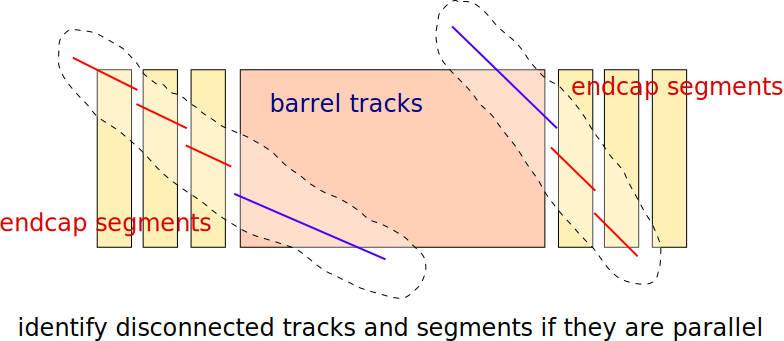
\includegraphics[width=0.75\linewidth]{identify_if_parallel}
\end{center}
\item If I understand correctly, CSC tracks have not been reconstructed due to moving disks: waiting for alignment

\item First exercise of prompt AlCaReco streams (practice for collisions)

\item First alignment in 2\_1\_X (all the configuration files had to be rewritten in Python)
\end{itemize}
\end{frame}

\begin{frame}
\frametitle{Closure of the endcaps}
\small
\begin{columns}
\column{0.8\linewidth}

$Z$ measurement versus time for YE+1, +2, +3

\includegraphics[width=\linewidth]{timeseries_YEp1.pdf}

\includegraphics[width=\linewidth]{timeseries_YEp2.pdf}

\includegraphics[width=\linewidth]{timeseries_YEp3.pdf}

\column{0.2\linewidth}

dotted line is nominal position

\vspace{0.5 cm}
YE+1 was closed from the start

\vspace{0.5 cm}
YE+2 and +3 were closed later

\vspace{0.5 cm}
is there a record for comparison (better precision)?

\end{columns}
\end{frame}

\begin{frame}
\frametitle{Disappearance of minus-side data}
\small
\begin{columns}
\column{0.8\linewidth}

$Z$ measurement versus time for YE-1, -2, -3

\includegraphics[width=\linewidth]{timeseries_YEm1.pdf}

\includegraphics[width=\linewidth]{timeseries_YEm2.pdf}

\includegraphics[width=\linewidth]{timeseries_YEm3.pdf}

\column{0.2\linewidth}

only have early block, before minus-side was closed

\vspace{0.5 cm}
I'm pretty sure the loss of data happened upstream of AlCaReco

\vspace{0.5 cm}
has anyone else seen this?

\end{columns}
\end{frame}

\begin{frame}
\frametitle{Tracker-to-muon alignments}
\small

\begin{itemize}\setlength{\itemsep}{0.3 cm}
\item Problem with the globalMuon AlCaRecos: tracker hit positions are
  no longer stored, they {\it must} be re-computed from clusters

\item MuonSelector didn't add clusters associated with tracks (but
  Javier just implemented that, awaiting validation)--- however,
  cosmic ray AlCaRecos already have {\it all} tracker clusters

\item We need to reconfigure alignment procedure to use this
  information: not a solved problem yet, but it might be a
  configuration-file change (hopefully)

\item In progress!

\item Due to setback, manpower issues, and a lot of things happening
  at once, our first tracker-to-muon alignment may be in CRAFT (which
  is all we promised back in the spring)

\end{itemize}
\end{frame}

\begin{frame}
\frametitle{Final comments}
\small
\begin{itemize}\setlength{\itemsep}{0.3 cm}

\item CRUZET-4 global tag due tomorrow; constants can be delivered on
  that timescale (I have the ntuples)

\item My information is partial and low-statistics: if there's a
  record of disk positions, I'll cross-check what I can and use the
  best information to construct constants

This moving-disks era is a very special case for alignment

\item All CRUZETs due next Tuesday: that leaves only CRUZET-3 (use
  Michael's skims as a starting point)

\end{itemize}

\vfill
\begin{itemize}
\item CSC Overlaps procedure is progressing: more detail at a later meeting
\end{itemize}

\label{numpages}
\end{frame}

%% \section*{First section}
%% \begin{frame}
%% \begin{center}
%% \Huge \textcolor{blue}{First section}
%% \end{center}
%% \end{frame}

\end{document}
